%%%%%%%%%%%%%%%%%%%%%%%%%%%%%%%%%%%%%%%%%%
%                                        %
% Szablon pracy dyplomowej magisterskiej % 
%                                        %
%%%%%%%%%%%%%%%%%%%%%%%%%%%%%%%%%%%%%%%%%%



\documentclass[a4paper,twoside,12pt]{book}
\usepackage[utf8]{inputenc}                                      
\usepackage[T1]{fontenc}  
\usepackage{amsmath,amsfonts,amssymb,amsthm}
\usepackage[british,polish]{babel} 
\usepackage{indentfirst}
\usepackage{lmodern}
\usepackage{graphicx} 
\usepackage{hyperref}
\usepackage{booktabs}
\usepackage{tikz}
\usepackage{pgfplots}
\usepackage{mathtools}
\usepackage[page]{appendix} % toc,
\renewcommand{\appendixtocname}{Dodatki}
\renewcommand{\appendixpagename}{Dodatki}
\renewcommand{\appendixname}{Dodatek}

\usepackage{setspace}
\onehalfspacing


\frenchspacing

\usepackage{listings}
\lstset{
	language={},
	basicstyle=\ttfamily,
	keywordstyle=\lst@ifdisplaystyle\color{blue}\fi,
	commentstyle=\color{gray}
}

%%%%%%%%%

%%%% TODO LIST GENERATOR %%%%%%%%%

%\usepackage{tikz}
%\usepackage{manfnt}   % dangerous sign 
\usepackage{color}
\definecolor{brickred}      {cmyk}{0   , 0.89, 0.94, 0.28}

\makeatletter \newcommand \kslistofremarks{\section*{Uwagi} \@starttoc{rks}}
  \newcommand\l@uwagas[2]
    {\par\noindent \textbf{#2:} %\parbox{10cm}
{#1}\par} \makeatother


\newcommand{\ksremark}[1]{%
{%\marginpar{\textdbend}
{\color{brickred}{[#1]}}}%
\addcontentsline{rks}{uwagas}{\protect{#1}}%
}

\newcommand{\comma}{\ksremark{przecinek}}
\newcommand{\nocomma}{\ksremark{bez przecinka}}
\newcommand{\styl}{\ksremark{styl}}
\newcommand{\ortografia}{\ksremark{ortografia}}
\newcommand{\fleksja}{\ksremark{fleksja}}
\newcommand{\pauza}{\ksremark{pauza `--', nie dywiz `-'}}
\newcommand{\kolokwializm}{\ksremark{kolokwializm}}

%%%%%%%%%%%%%% END OF TODO LIST GENERATOR %%%%%%%%%%%

%%%%%%%%%%%% ZYWA PAGINA %%%%%%%%%%%%%%%
% brak kapitalizacji zywej paginy
\usepackage{fancyhdr}
\pagestyle{fancy}
\fancyhf{}
\fancyhead[LO]{\nouppercase{\it\rightmark}}
\fancyhead[RE]{\nouppercase{\it\leftmark}}
\fancyhead[LE,RO]{\it\thepage}


\fancypagestyle{tylkoNumeryStron}{%
   \fancyhf{} 
   \fancyhead[LE,RO]{\it\thepage}
}

\fancypagestyle{NumeryStronNazwyRozdzialow}{%
   \fancyhf{} 
   \fancyhead[LO]{\nouppercase{\it\rightmark}}
   \fancyhead[RE]{\nouppercase{\it\leftmark}}
   \fancyhead[LE,RO]{\it\thepage}
}


%%%%%%%%%%%%% OBCE WTRETY  
\newcommand{\obcy}[1]{\emph{#1}}
\newcommand{\ang}[1]{{\selectlanguage{british}\obcy{#1}}}
%%%%%%%%%%%%%%%%%%%%%%%%%%%%%

% polskie oznaczenia funkcji matematycznych
\renewcommand{\tan}{\operatorname {tg}}
\renewcommand{\log}{\operatorname {lg}}

% jeszcze jakies drobiazgi

\newcounter{stronyPozaNumeracja}

\newcommand{\hcancel}[1]{%
    \tikz[baseline=(tocancel.base)]{
        \node[inner sep=0pt,outer sep=0pt] (tocancel) {#1};
        \draw[red] (tocancel.south west) -- (tocancel.north east);
    }%
}%

\newcommand{\miesiac}{%
  \ifcase\the\month
  \or styczeń% 1
  \or luty% 2
  \or marzec% 3
  \or kwiecień% 4
  \or maj% 5
  \or czerwiec% 6
  \or lipiec% 7
  \or sierpień% 8
  \or wrzesień% 9
  \or październik% 10
  \or listopad% 11
  \or grudzień% 12
  \fi}


%%%%%%%%%%%%%%%%%%%%%%%%%%%%%%%%%%%%%%%%%%%%%%
%%%%%%%%%%%%%%%%%%%%%%%%%%%%%%%%%%%%%%%%%%%%%%
%%%%%%%%%%%%%%%%%%%%%%%%%%%%%%%%%%%%%%%%%%%%%%
%%%%%%%%%%%%%%%%%%%%%%%%%%%%%%%%%%%%%%%%%%%%%%
%%%%%%%%%%%%%%%%%%%%%%%%%%%%%%%%%%%%%%%%%%%%%%
%%%%%%%%%%%%%%%%%%%%%%%%%%%%%%%%%%%%%%%%%%%%%%
%%%%%%%%%%%%%%%%%%%%%%%%%%%%%%%%%%%%%%%%%%%%%%
%%%%%%%%%%%%%%%%%%%%%%%%%%%%%%%%%%%%%%%%%%%%%%


\newcommand{\autor}{Mateusz Trzeciak}
\newcommand{\promotor}{dr inż. Karolina Nurzyńska}
\newcommand{\tytul}{Określenie wieku twarzy na podstawie tekstury}


\begin{document}
%\kslistofremarks 
	
%%%%%%%%%%%%%%%%%%  STRONA TYTULOWA %%%%%%%%%%%%%%%%%%%
\pagestyle{empty}
\sffamily

\noindent

\begin{center}
    \large
    Politechnika Śląska\\
    Wydział Automatyki, Elektroniki i~Informatyki \\ 
    kierunek: informatyka
\end{center}

\vfill\vfill
\begin{center}
    \large
    \autor
\end{center}

\vfill
\begin{center}
   \LARGE\bfseries \tytul
\end{center}

\vfill
\begin{center}
    \large
    praca dyplomowa magisterska
\end{center}

\vfill\vfill\vfill
\begin{center}
    \large
    \begin{tabular}{ll}
    promotor: & \promotor \\
   % konsultant: & \konsultant \\ % jezeli nie ma, zakomentowac
    \end{tabular}

\end{center}

\vfill
\begin{center}
\large
   Gliwice,  \miesiac\ \the\year
\end{center}

\cleardoublepage
 

\rmfamily
\normalfont

%%%%%%%%%%%%%%%%%%%%% oswiadczenie o udostępnianiu pracy dyplomowej %%%%%%%%%%%%%%%%%%%
\cleardoublepage

\begin{flushright}
załącznik nr 2 do zarz. nr 97/08/09 
\end{flushright}

\vfill  

\begin{center}
\Large\bfseries Oświadczenie
\end{center}

\vfill

Wyrażam  zgodę / Nie wyrażam zgody*  na  udostępnienie  mojej  pracy  dyplomowej / rozprawy doktorskiej*.

\vfill

Gliwice, dnia \today

\vfill

\rule{0.5\textwidth}{0cm}\dotfill 

\rule{0.5\textwidth}{0cm}
\begin{minipage}{0.45\textwidth}
{\begin{center}(podpis)\end{center}}
\end{minipage} 

\vfill

\rule{0.5\textwidth}{0cm}\dotfill 

\rule{0.5\textwidth}{0cm}
\begin{minipage}{0.45\textwidth}
{\begin{center}\rule{0mm}{5mm}(poświadczenie wiarygodności podpisu przez Dziekanat)\end{center}}
\end{minipage}


\vfill

* podkreślić właściwe

 


%%%%%%%%%%%%%%%%%%%%% oswiadczenie promotora o spełnieniu wymagań formalnych %%%%%%%%%%%%%%%%%%%
\cleardoublepage

\rule{1cm}{0cm}

\vfill  

\begin{center}
\Large\bfseries Oświadczenie promotora
\end{center}

\vfill

Oświadczam, że praca „\tytul” spełnia wymagania formalne pracy dyplomowej magisterskiej.

\vfill



\vfill

Gliwice, dnia \today

\rule{0.5\textwidth}{0cm}\dotfill 

\rule{0.5\textwidth}{0cm}
\begin{minipage}{0.45\textwidth}
{\begin{center}(podpis promotora)\end{center}}
\end{minipage} 

\vfill

%\rule{0.5\textwidth}{0cm}\dotfill 
%
%\rule{0.5\textwidth}{0cm}
%\begin{minipage}{0.45\textwidth}
%{\begin{center}\rule{0mm}{5mm}(poświadczenie wiarygodności podpisu przez Dziekanat)\end{center}}
%\end{minipage}
%
%
%\vfill

 

\cleardoublepage


%%%%%%%%%%%%%%%%%% SPIS TRESCI %%%%%%%%%%%%%%%%%%%%%%
\pagenumbering{Roman}
\pagestyle{tylkoNumeryStron}
\tableofcontents

%%%%%%%%%%%%%%%%%%%%%%%%%%%%%%%%%%%%%%%%%%%%%%%%%%%%%
\setcounter{stronyPozaNumeracja}{\value{page}}
\mainmatter
\pagestyle{NumeryStronNazwyRozdzialow}

%%%%%%%%%%%%%% wlasciwa tresc pracy %%%%%%%%%%%%%%%%%

\chapter{Wstęp}

%\begin{itemize}
%\item wprowadzenie w problem/zagadnienie 
%\item osadzenie problemu w dziedzinie 
%\item cel pracy 
%\item zakres pracy 
%\item zwięzła charakterystyka rozdziałów 
%\item jednoznaczne określenie wkładu autora
%\end{itemize}
Wiek jest cechą, którą niałatwo odczytać człowiekowi z czyjejś twarzy. Twarz może wyglądać inaczej u osoby, która dba o siebie, a inaczej u osoby, która nie dba. Dla komputera rozpoznawanie wieku jest trudniejsze niż dla człowieka. Dlatego do wyznaczania wieku z pomocą programu komputerowego należy podchodzić z dystansem. Mimo trudności programiści i naukowcy udoskonalają algorytmy, tak aby ocena wieku danej osoby była coraz lepsza.

Istnieje wiele sposobów wyznaczania wieku. Większość metod skupia się na analizie tekstury twarzy. Idąc dalej - z obrazu danej osoby lub jego części np tułowia musi zostać wyodrebniona twarz. Wyodrębnianie twarzy z danej tekstury można uzyskać dzięki specjalnej technice komputerowej zwanej rozpoznawaniem obrazu. Rozpoznawanie obrazu zwane również wizją komputerową to przetwarzanie grafiki, polegające na wyodrębnianiu z niej jakichś szczegółów. Mogą to być osoby, pojazdy, przedmioty itp. (Rys. \ref{fig.rozpoznawanieObiektow})

\begin{figure}
	\centering
	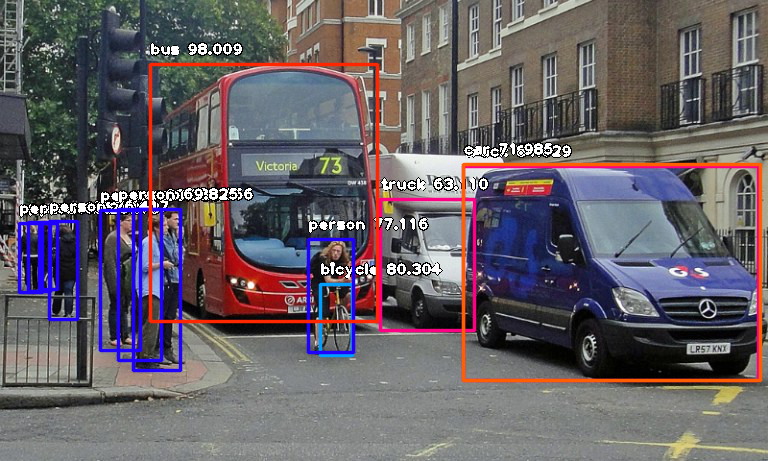
\includegraphics[width=11cm]{Obrazy/rozpoznawanieObiektow} 
	\caption{Przykład rozpoznawania obiektów na zdjęciu ulicy. \cite{rozpoznawanieObiektow}}.
	\label{fig.rozpoznawanieObiektow}
\end{figure}

Można znaleźć wiele witryn internetowych, które udostępniają interfejsy programistyczne umożliwiające zaimplementowanie rozpoznawania wieku z obrazu. Istnieją algorytmy przetwarzania obrazu, które oprócz wieku wyznaczają z pewnym prawdopodobieństwem płeć danej osoby. Oprócz płci mogą one także wyznaczać samopoczucie, czy dana osoba się uśmiecha oraz czy posiada okulary.

Z weryfikacją wieku danej osoby można się spotkać przed wejściem do niektórych miejsc np. klub nocny. Większość osób musi okazać ważny dowód osobisty. Co generuje duże kolejki do wejścia. Aplikację analizujące wiek na podstawie obrazu twarzy z kamery, przed wejściem do takich miejsc znacząco usprawniłyby weryfikację wieku.
Rozpoznawanie wieku może być wykorzystywane przy analizie średniego wieku ludzi w jakimś miejscu np. podczas demonstracji.

 Wiele gier posiada treści nieodpowiednie dla młodszych użytkowników. Możliwe jest stosowanie technologii wykrywania wieku użytkownika przed udostępnieniem mu treści, która wymaga odpowiedniego wieku.
 
  Można znaleźć o wiele więcęj potencjalnych zastosowań przetwarzania obrazu oraz rozpoznawania wieku na podstawie tekstury (obrazu) twarzy. Z biegiem lat z pewnością będzie można zauważyć rozwój tej dziedziny.



\chapter{[Analiza tematu]}

\begin{itemize}
\item analiza tematu
\item wprowadzenie do dziedziny (\ang{state of the art}) – sformułowanie problemu, 
\item poszerzone studia literaturowe, przegląd literatury tematu (należy wskazać źródła wszystkich informacji zawartych w pracy)
\item opis znanych rozwiązań, algorytmów, osadzenie pracy w kontekście
\item Tytuł rozdziału jest często zbliżony do tematu pracy. 
\item Rozdział jest wysycony cytowaniami do literatury \cite{bib:artykul,bib:ksiazka,bib:konferencja}.
\end{itemize}




\chapter{[Przedmiot pracy]}

\begin{itemize}
\item rozwiązanie zaproponowane przez dyplomanta
\item analiza teoretyczna rozwiązania
\item uzasadnienie wyboru zastosowanych metod, algorytmów, narzędzi
\end{itemize}

\chapter{Badania}

 

Rozdział przedstawia przeprowadzone badania. Jest to zasadnicza część i~musi wyraźnie dominować w~pracy.
Badania i analizę wyników należy przeprowadzić, tak jak jest przyjęte w środowisku naukowym (na przykład korzystanie z danych benchmarkowych, walidacja krzyżowa, zapewnienie powtarzalności testów itd). 

\section{Metodyka badań}

\begin{itemize}
\item opis metodyki badań
\item opis stanowiska badawczego (opis interfejsu aplikacji badawczych -- w~załączniku)
\end{itemize}


\section{Zbiory danych}

\begin{itemize}
\item opis danych
\end{itemize}


\section{Wyniki}

\begin{itemize}
\item prezentacja wyników, opracowanie i poszerzona dyskusja  wyników, wnioski
\end{itemize}


\begin{figure}
\centering
\begin{tikzpicture}
\begin{axis}[
    y tick label style={
        /pgf/number format/.cd,
            fixed,   % po zakomentowaniu os rzednych jest indeksowana wykladniczo
            fixed zerofill, % 1.0 zamiast 1
            precision=1,
        /tikz/.cd
    },
    x tick label style={
        /pgf/number format/.cd,
            fixed,
            fixed zerofill,
            precision=2,
        /tikz/.cd
    }
]
\addplot [domain=0.0:0.1] {rnd};
\end{axis} 
\end{tikzpicture}
\caption{Podpis rysunku po rysunkiem.}
\label{fig:2}
\end{figure}

\begin{table}
\centering
\caption{Opis tabeli nad nią.}
\label{id:tab:wyniki}
\begin{tabular}{rrrrrrrr}
\toprule
	         &                                     \multicolumn{7}{c}{metoda}                                      \\
	         \cmidrule{2-8}
	         &         &         &        \multicolumn{3}{c}{alg. 3}        & \multicolumn{2}{c}{alg. 4, $\gamma = 2$} \\
	         \cmidrule(r){4-6}\cmidrule(r){7-8}
	$\zeta$ &     alg. 1 &   alg. 2 & $\alpha= 1.5$ & $\alpha= 2$ & $\alpha= 3$ &   $\beta = 0.1$  &   $\beta = -0.1$ \\
\midrule
	       0 &  8.3250 & 1.45305 &       7.5791 &    14.8517 &    20.0028 & 1.16396 &                       1.1365 \\
	       5 &  0.6111 & 2.27126 &       6.9952 &    13.8560 &    18.6064 & 1.18659 &                       1.1630 \\
	      10 & 11.6126 & 2.69218 &       6.2520 &    12.5202 &    16.8278 & 1.23180 &                       1.2045 \\
	      15 &  0.5665 & 2.95046 &       5.7753 &    11.4588 &    15.4837 & 1.25131 &                       1.2614 \\
	      20 & 15.8728 & 3.07225 &       5.3071 &    10.3935 &    13.8738 & 1.25307 &                       1.2217 \\
	      25 &  0.9791 & 3.19034 &       5.4575 &     9.9533 &    13.0721 & 1.27104 &                       1.2640 \\
	      30 &  2.0228 & 3.27474 &       5.7461 &     9.7164 &    12.2637 & 1.33404 &                       1.3209 \\
	      35 & 13.4210 & 3.36086 &       6.6735 &    10.0442 &    12.0270 & 1.35385 &                       1.3059 \\
	      40 & 13.2226 & 3.36420 &       7.7248 &    10.4495 &    12.0379 & 1.34919 &                       1.2768 \\
	      45 & 12.8445 & 3.47436 &       8.5539 &    10.8552 &    12.2773 & 1.42303 &                       1.4362 \\
	      50 & 12.9245 & 3.58228 &       9.2702 &    11.2183 &    12.3990 & 1.40922 &                       1.3724 \\
\bottomrule
\end{tabular}
\end{table}  



\chapter{Podsumowanie}
\begin{itemize}
\item syntetyczny opis wykonanych prac
\item wnioski
\item możliwość rozwoju, kontynuacji prac, potencjalne nowe kierunki
\item Czy cel pracy zrealizowany? 
\end{itemize}


%%%%%%%%%%%%%%%%%%%%%%%%%%%%%%%%%%%%%%%%%%
\backmatter
\pagenumbering{Roman}
\stepcounter{stronyPozaNumeracja}
\setcounter{page}{\value{stronyPozaNumeracja}}

\pagestyle{tylkoNumeryStron}

%%%%%%%%%%% bibliografia %%%%%%%%%%%%
\bibliographystyle{plplain}
\bibliography{bibliografia}

%%%%%%%%%  DODATKI %%%%%%%%%%%%%%%%%%% 

\begin{appendices} 


\chapter*{Dokumentacja techniczna}

\chapter*{Spis skrótów i symboli}

\begin{itemize}
\item[DNA] kwas deoksyrybonukleinowy (ang. \ang{deoxyribonucleic acid})
\item[MVC] model -- widok -- kontroler (ang. \ang{model--view--controller}) 
\item[$N$] liczebność zbioru danych
\item[$\mu$] stopnień przyleżności do zbioru
\item[$\mathbb{E}$] zbiór krawędzi grafu
\item[$\mathcal{L}$] transformata Laplace'a 
\end{itemize}


 

\chapter*{Zawartość dołączonej płyty}

Do pracy dołączona jest płyta CD z~następującą zawartością:
\begin{itemize}
\item praca w~formacie \texttt{pdf},
\item źródła programu,
\item zbiory danych użyte w~eksperymentach.
\end{itemize}

\listoffigures
\listoftables
	
\end{appendices}


\end{document}


%% Finis coronat opus.